\section{Bloque 3. Algoritmos de consulta: Deutsch, Deutsch-Jozsa y Bernstein-Vazirani}\label{sec:bloque_3}

\subsection{Ejercicio 3.1: Algoritmo de Deutsch}
En el siguiente ejercicio se implementa el Algoritmo de Deutsch para cada uno de los casos de funciones binarias de una variable.

\textbf{Oráculo a.} Oráculo de la función constante 0, $f(x) = 0$. Es una función constante, por lo tanto tras ejecutar el algoritmo
de Deutsch se debería de medir en el qubit de dato $q_0$ el estado $\ket{0}$. En la Figura~\ref{fig:bloque3_e3_1_a} se observa el circuito del algoritmo
y el histograma de la medida sobre el qubit de dato $q_0$. La simulación coincide con la predicción. 

\begin{figure}[h]
    \centering
    \begin{subfigure}{0.48\textwidth}
        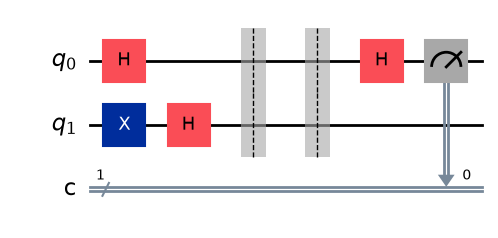
\includegraphics[width=\textwidth]{imagenes/bloque3/e3_1_circuito_a.png}
        \caption{}
    \end{subfigure}
    \hfill
    \begin{subfigure}{0.48\textwidth}
        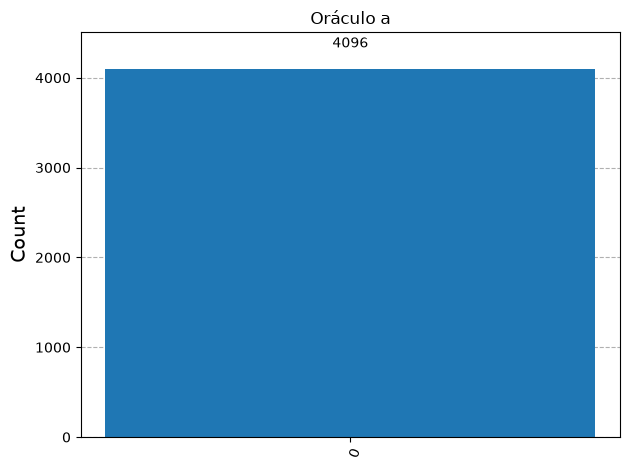
\includegraphics[width=0.7\textwidth]{imagenes/bloque3/e3_1_histograma_a.png}
        \caption{}
    \end{subfigure}
    \caption{(a): Circuito construido para Oráculo a. \\
    (b): Histograma del algoritmo de Deutsch para el Oráculo a.}\label{fig:bloque3_e3_1_a}
\end{figure}


\textbf{Oráculo b.} Oráculo de la función constante 1, $f(x) = 1$. Es una función constante, por lo tanto tras ejecutar el algoritmo
de Deutsch se debería de medir en el qubit de dato $q_0$ el estado $\ket{0}$. En la Figura~\ref{fig:bloque3_e3_1_b} se observa el circuito del algoritmo
y el histograma de la medida sobre el qubit de dato $q_0$. La simulación coincide con la predicción. 

\begin{figure}[h]
    \centering
    \begin{subfigure}{0.48\textwidth}
        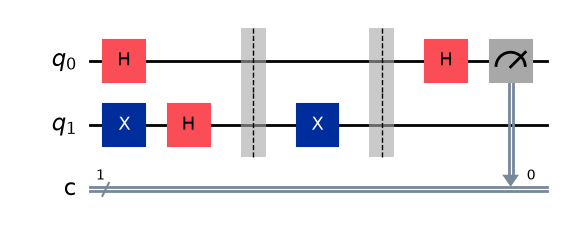
\includegraphics[width=\textwidth]{imagenes/bloque3/e3_1_circuito_b.png}
        \caption{}
    \end{subfigure}
    \hfill
    \begin{subfigure}{0.48\textwidth}
        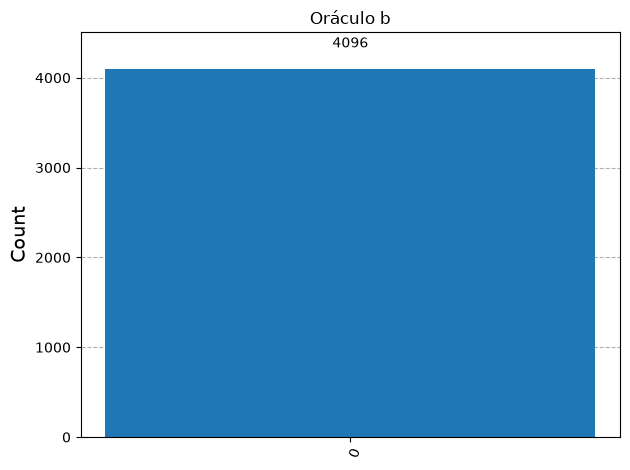
\includegraphics[width=0.7\textwidth]{imagenes/bloque3/e3_1_histograma_b.png}
        \caption{}
    \end{subfigure}
    \caption{(a): Circuito construido para Oráculo b. \\
    (b): Histograma del algoritmo de Deutsch para el Oráculo b.}\label{fig:bloque3_e3_1_b}
\end{figure}

\textbf{Oráculo c.} Oráculo de la función identidad $f(x) = x$. Es una función balanceada, por lo tanto tras ejecutar el algoritmo
de Deutsch se debería de medir en el qubit de dato $q_0$ el estado $\ket{1}$. En la Figura~\ref{fig:bloque3_e3_1_c} se observa el circuito del algoritmo
y el histograma de la medida sobre el qubit de dato $q_0$. La simulación coincide con la predicción. 
\begin{figure}[h]
    \centering
    \begin{subfigure}{0.48\textwidth}
        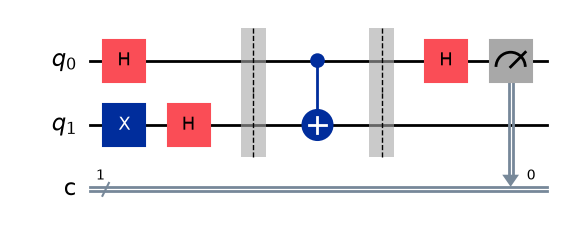
\includegraphics[width=\textwidth]{imagenes/bloque3/e3_1_circuito_c.png}
        \caption{}
    \end{subfigure}
    \hfill
    \begin{subfigure}{0.48\textwidth}
        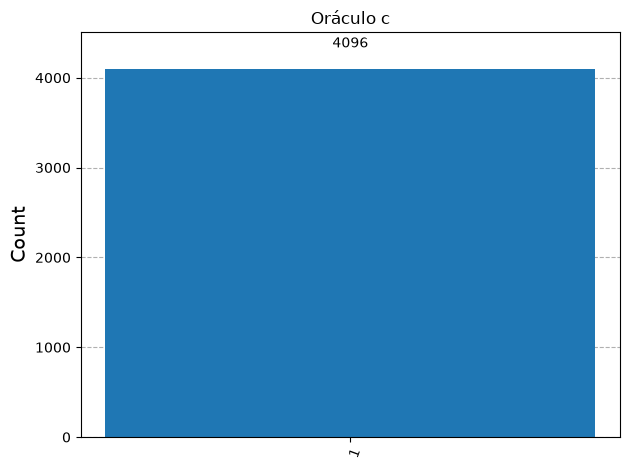
\includegraphics[width=0.7\textwidth]{imagenes/bloque3/e3_1_histograma_c.png}
        \caption{}
    \end{subfigure}
    \caption{(a): Circuito construido para Oráculo c. \\
    (b): Histograma del algoritmo de Deutsch para el Oráculo c.}\label{fig:bloque3_e3_1_c}
\end{figure}

\textbf{Oráculo d.} Oráculo de la función inversa, $f(x) = NOT(x)$. Es una función balanceada, por lo tanto tras ejecutar el algoritmo
de Deutsch se debería de medir en el qubit de dato $q_0$ el estado $\ket{1}$. En la Figura~\ref{fig:bloque3_e3_1_d} se observa el circuito del algoritmo
y el histograma de la medida sobre el qubit de dato $q_0$. La simulación coincide con la predicción. 

\begin{figure}[h]
    \centering
    \begin{subfigure}{0.48\textwidth}
        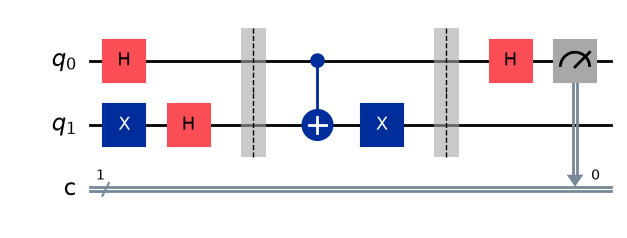
\includegraphics[width=\textwidth]{imagenes/bloque3/e3_1_circuito_d.png}
        \caption{}
    \end{subfigure}
    \hfill
    \begin{subfigure}{0.48\textwidth}
        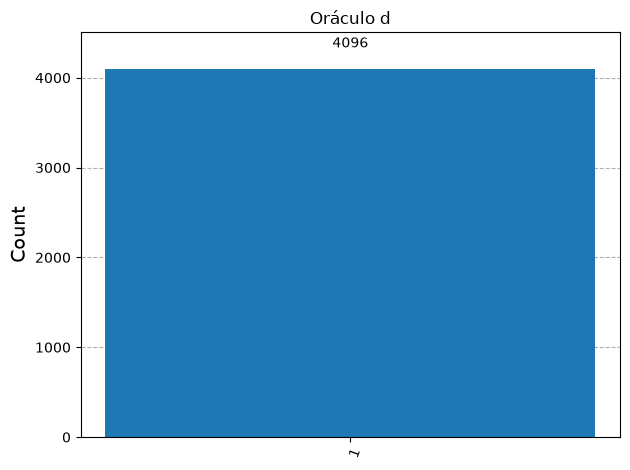
\includegraphics[width=0.7\textwidth]{imagenes/bloque3/e3_1_histograma_d.png}
        \caption{}
    \end{subfigure}
    \caption{(a): Circuito construido para Oráculo d. \\
    (b): Histograma del algoritmo de Deutsch para el Oráculo d.}\label{fig:bloque3_e3_1_d}
\end{figure}


\subsection{Ejercicio 3.2: Deutsch-Jozsa con \texorpdfstring{$n=2$}{n=2}}
En el siguiente ejercicio se implementa el algoritmo de Deutsch-Jozsa para una serie de funciones y se evalúa los histogramas de la simulación.

\textbf{Función a.} Función constante 0, $f(x_1, x_0) = 0$. En la Figura~\ref{fig:bloque3_e3_2_a} se muestra el oráculo para la 
función especificada en este apartado. Al ser una función constante, el valor medido en los qubits de datos tras la ejecución del algoritmo sería
$\ket{00}$ que efectivamente se cumple en el histograma mostrado en la Figura mencionada.

\begin{figure}[]
    \centering
    \begin{subfigure}{0.4\textwidth}
        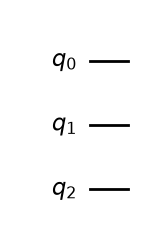
\includegraphics[width=0.4\textwidth]{imagenes/bloque3/e3_2_oraculo_a.png}
        \caption{}
    \end{subfigure}
    %\hfill
    \begin{subfigure}{0.4\textwidth}
        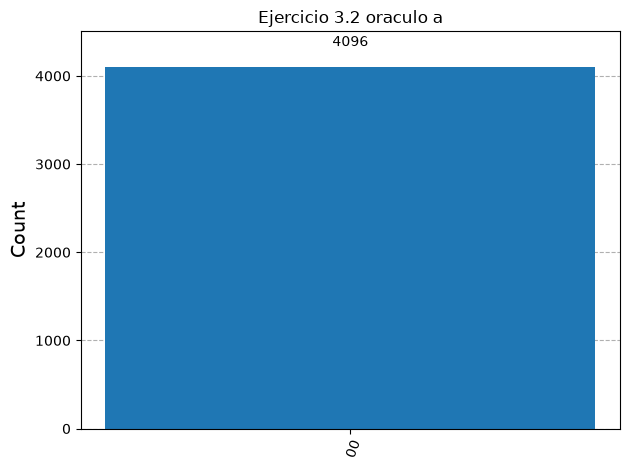
\includegraphics[width=0.75\textwidth]{imagenes/bloque3/e3_2_histograma_a.png}
        \caption{}
    \end{subfigure}
    \caption{(a): Circuito construido para Oráculo a. \\
    (b): Histograma del algoritmo de Deutsch-Jozsa para el Oráculo a.}\label{fig:bloque3_e3_2_a}
\end{figure}

\textbf{Función b.} Función $f(x_1, x_0) = x_1 \oplus x_0$. En la Figura~\ref{fig:bloque3_e3_2_b} se muestra el oráculo implementado
para esta función junto al histograma del resultado de la medida tras la ejecución del algoritmo. El resultado medido corresponde al estado
$\ket{11}$ lo que indica que la función es balanceada.

\begin{figure}[h]
    \centering
    \begin{subfigure}{0.4\textwidth}
        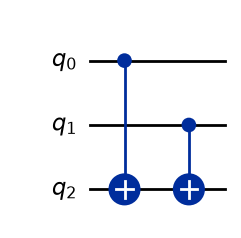
\includegraphics[width=0.5\textwidth]{imagenes/bloque3/e3_2_oraculo_b.png}
        \caption{}
    \end{subfigure}
    %\hfill
    \begin{subfigure}{0.4\textwidth}
        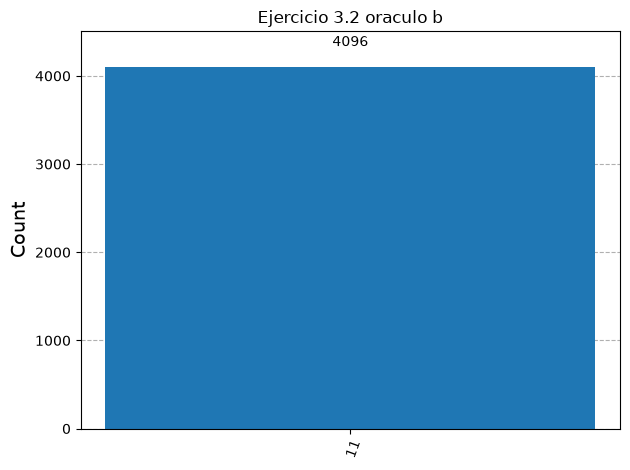
\includegraphics[width=0.75\textwidth]{imagenes/bloque3/e3_2_histograma_b.png}
        \caption{}
    \end{subfigure}
    \caption{(a): Circuito construido para Oráculo b. \\
    (b): Histograma del algoritmo de Deutsch-Jozsa para el Oráculo b.}\label{fig:bloque3_e3_2_b}
\end{figure}

\begin{figure}[h]
    \centering
    \begin{subfigure}{0.4\textwidth}
        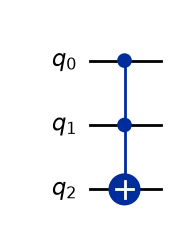
\includegraphics[width=0.45\textwidth]{imagenes/bloque3/e3_2_oraculo_c.png}
        \caption{}
    \end{subfigure}
    %\hfill
    \begin{subfigure}{0.4\textwidth}
        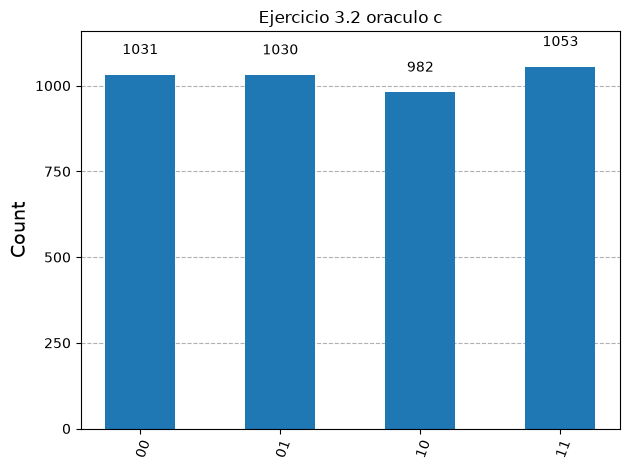
\includegraphics[width=0.75\textwidth]{imagenes/bloque3/e3_2_histograma_c.png}
        \caption{}
    \end{subfigure}
    \caption{(a): Circuito construido para Oráculo c. \\
    (b): Histograma del algoritmo de Deutsch-Jozsa para el Oráculo c.}\label{fig:bloque3_e3_2_c}
\end{figure}

\textbf{Función c.} Función $f(x_1, x_0) = x_1 \land x_0$. En la
Figura~\ref{fig:bloque3_e3_2_c} se muestra el oráculo implementado para
esta función junto al histograma del resultado de la medida tras la
ejecución del algoritmo. El oráculo se implementa con una puerta Toffoli
que suma la operación AND de los dos primeros qubits sobre el último. En
el histograma aparecen las cuatro cadenas, entre ellas $\ket{00}$ y otras
que no lo son.

\textbf{Predicción y por qué no se puede concluir.} Para
$f(x_1,x_0)=x_1\wedge x_0$ solo hay un $1$ entre las cuatro entradas
($f(11)=1$), de modo que $f$ no es constante ni balanceada y no cumple la
promesa de Deutsch-Jozsa. La amplitud de la cadena $z=z_1z_0$ al final
del algoritmo es
\[
  \alpha_z=\frac14\sum_{x_1,x_0}(-1)^{\,f(x_1,x_0)\,\oplus\,(z_1x_1\oplus z_0x_0)},
\]
que da $\alpha_{00}=\alpha_{01}=\alpha_{10}=\tfrac12$ y
$\alpha_{11}=-\tfrac12$ (por ejemplo,
$\alpha_{00}=\tfrac14(1+1+1-1)=\tfrac12$). Por tanto, las cuatro cadenas
se miden con probabilidad $|\alpha_z|^2=1/4$. La simulación lo confirma
(Figura~\ref{fig:bloque3_e3_2_c}b): se obtienen 1031, 1030, 982 y 1053
conteos de 4096 frente a los 1024 esperados ($\chi^2=2{,}63$ con
3 grados de libertad, $p=0{,}453$).

Si $f$ fuese constante se mediría $00$ con probabilidad $1$, y si fuese
balanceada no se mediría nunca ($\alpha_{00}=0$). Aquí $00$ aparece con
probabilidad $1/4$, que no corresponde a ninguno de los dos casos, y el
resto de cadenas tampoco permite distinguirlos. Como la promesa no se
cumple, la medida carece de interpretación y no se puede extraer ninguna
conclusión de ella sobre el tipo de $f$.

\subsection{Ejercicio 3.3: Bernstein-Vazirani}\label{subsection:ejercicio3_3}
En este ejercicio se ha implementado el algoritmo de Bernstein-Vazirani para obtener una clave $a = 1010$, construyendo el oráculo
correspondiente. En la Figura~\ref{fig:bloque3_e3_3_a1} se puede observar el oráculo implementado para dicha clave $a$. También se ha simulado
el algoritmo con un único \textit{shot} y se ha podido conseguir la clave, tal y como se pide en el enunciado.

\textbf{Observación: } A la hora de realizar la medida se ha invertido el orden de los bits clásicos a los que corresponden cada qubit. Es decir, 
al qubit $q_0$ se le ha asignado el bit clásico más significativo en la medida, y $q_3$ (el más significativo) se le ha asignado el bit clásico 
menos significativo. La implementación del oráculo se ha realizado teniendo la notación contraria de qubits a la de Qiskit, por lo que la inversión
del orden nos permite tener la notación correcta en los resultados de medida.
\begin{figure}[h]
    \centering
    \begin{subfigure}{0.4\textwidth}
        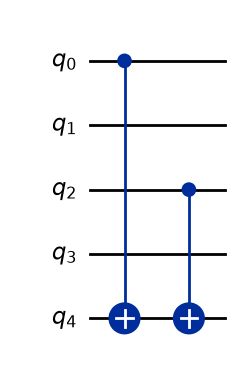
\includegraphics[width=0.5\textwidth]{imagenes/bloque3/e3_3_oraculo_a1.png}
        \caption{}
    \end{subfigure}
    %\hfill
    \begin{subfigure}{0.4\textwidth}
        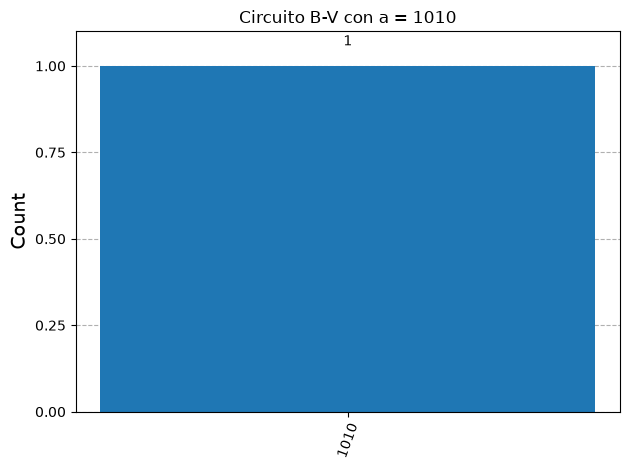
\includegraphics[width=0.8\textwidth]{imagenes/bloque3/e3_3_histograma_a1.png}
        \caption{}
    \end{subfigure}
    \caption{(a): Oráculo para la clave $a = 1010$. \\
    (b): Histograma de la ejecución del algoritmo para obtener la clave $a = 1010$}\label{fig:bloque3_e3_3_a1}
\end{figure}

Por otro lado, como segunda prueba, se ha escogido otra clave $a = 1101$ y se ha implementado el algoritmo. En la Figura~\ref{fig:bloque3_e3_3_a2}
se incluye el oráculo correspondiente junto al histograma de la ejecución con un único shot. Nuevamente se consigue obtener la clave secreta.

\begin{figure}[h]
    \centering
    \begin{subfigure}{0.4\textwidth}
        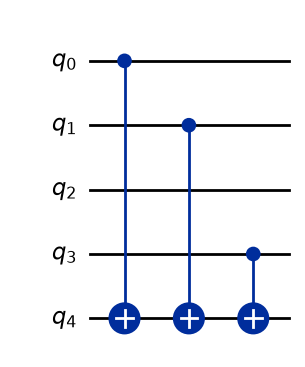
\includegraphics[width=0.5\textwidth]{imagenes/bloque3/e3_3_oraculo_a2.png}
        \caption{}
    \end{subfigure}
    %\hfill
    \begin{subfigure}{0.4\textwidth}
        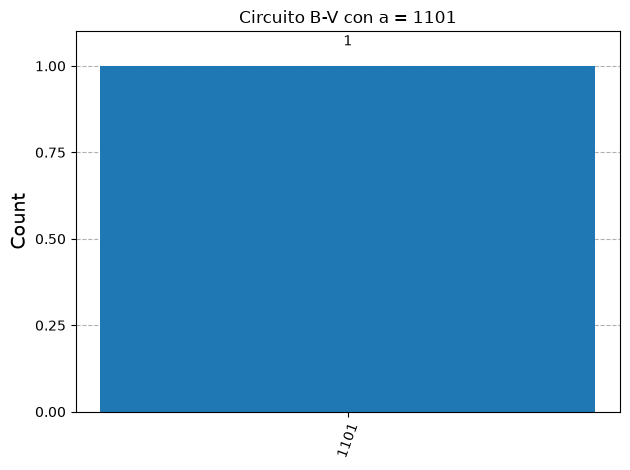
\includegraphics[width=0.8\textwidth]{imagenes/bloque3/e3_3_histograma_a2.png}
        \caption{}
    \end{subfigure}
    \caption{(a): Oráculo para la clave $a = 1101$. \\
    (b): Histograma de la ejecución del algoritmo para obtener la clave $a = 1101$}\label{fig:bloque3_e3_3_a2}
\end{figure}



\subsection{Ejercicio E1: Deutsch-Jozsa con un oráculo dado}
En este ejercicio se implementa el algoritmo de Deutsch-Jozsa para un oráculo dado y se quiere determinar qué tipo de función 
$f(x_0, x_1)$ corresponde (constante o balanceada). En la Figura~\ref{fig:bloque3_e1_algoritmo_df} se muestra el oráculo detallado
en el enunciado y el circuito que implementa el Algoritmo de Deutsch-Jozsa correspondiente.

\begin{figure}[h]
    \centering
    \begin{subfigure}{0.48\textwidth}
        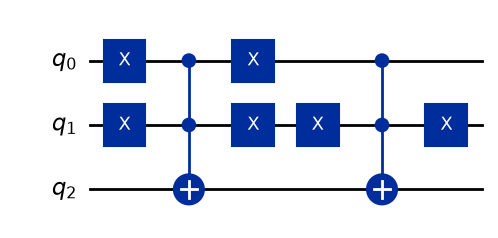
\includegraphics[width=0.9\textwidth]{imagenes/bloque3/e1_oraculo_df.png}
        \caption{}
    \end{subfigure}
    %\hfill
    \begin{subfigure}{0.48\textwidth}
        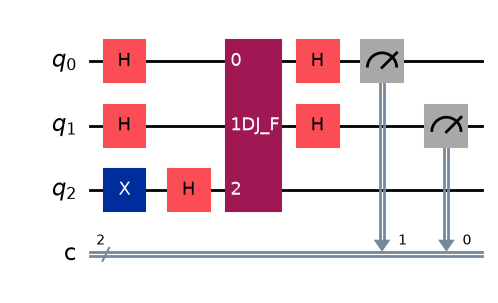
\includegraphics[width=0.9\textwidth]{imagenes/bloque3/e1_circuito.png}
        \caption{}
    \end{subfigure}
    \caption{(a): Oráculo $DJ\_F$ del enunciado. \\
    (b): Circuito que implementa el algoritmo de Deutsch-Jozsa}\label{fig:bloque3_e1_algoritmo_df}
\end{figure}

Tras simular el circuito, se mide el estado $\ket{01}$ que aparece en la Figura~\ref{fig:bloque3_e1_histograma_algoritmo}. Se ha realizado la misma inversión
del orden de los bits clásicos en la medida respecto de los qubits al igual que en el ejercicio anterior. Por lo tanto, el estado medido es $\ket{q_0, q_1} = \ket{01}$.

Con esta medición, de acuerdo a la formulación del algoritmo, se puede deducir que la amplitud del estado $\ket{00}$ es $0$, por lo que se puede
concluir que la función $f$ es \textbf{balanceada}. 
\begin{figure}
    \centering
    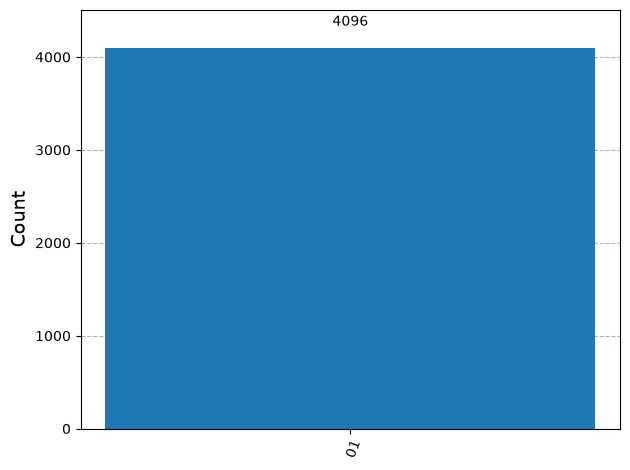
\includegraphics[width=0.35\textwidth]{imagenes/bloque3/e1_histograma_algoritmo.png}
    \caption{Histograma de la ejecución del algoritmo de Deutsch-Jozsa para el oráculo $DJ\_F$}\label{fig:bloque3_e1_histograma_algoritmo}
\end{figure}

Por otro lado, para obtener la tabla de verdad de la función $f$ se ha simulado el oráculo para cada una de las cuatro entradas
de la base computacional de los qubits $q_0, q_1$. Para evaluar la salida para cada entrada se ha inicializado $\ket{q_2} = \ket{0}$.
En la Figura~\ref{fig:bloque3_e1_histogramas} se puede visualizar el valor de las salidas de $f$ para cada una de las $4$ entradas
de la base computacional tras simular por separado el oráculo. Con ello podemos construir la tabla de verdad de $f$ y se deduce 
que la función simplificada es: $f(x_0, x_1) = \overline{x_1}$ (la barra denota que $f$ vale $1$ cuando $x_1 = 0$).
\begin{table}[htbp]
    \centering
    \begin{tabular}{c c c c}
        \toprule
        $x_0$ & $x_1$ & $x$ & $f(x)$ \\
        \midrule
        0 & 0 & 0 & 1 \\
        0 & 1 & 1 & 0 \\
        1 & 0 & 2 & 1 \\
        1 & 1 & 3 & 0 \\
        \bottomrule
    \end{tabular}
    \caption{Tabla de verdad de la función $f$.}\label{tab:bloque3_e1_tablaverdad}
\end{table}

\begin{figure}[htbp]
    \centering
    \begin{subfigure}{0.4\textwidth}
        \centering
        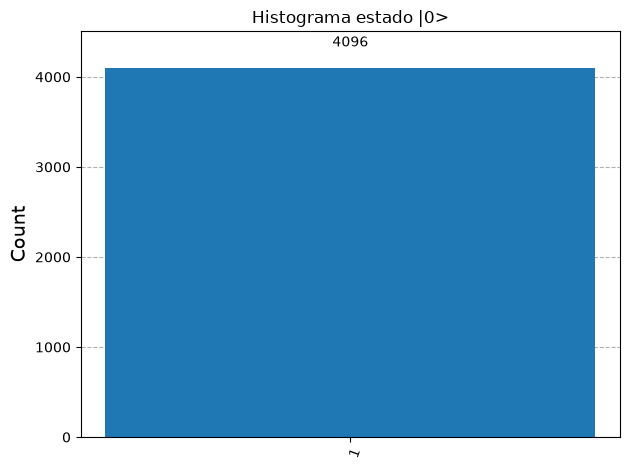
\includegraphics[width=\textwidth]{imagenes/bloque3/e1_histograma_f00.png}
        \caption{}
    \end{subfigure}
    \hfill
    \begin{subfigure}{0.4\textwidth}
        \centering
        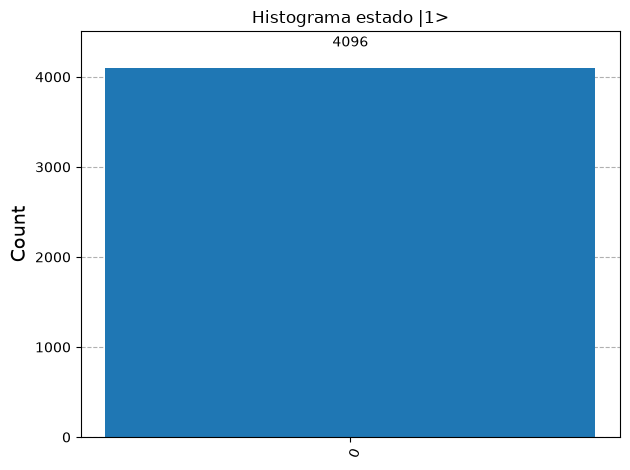
\includegraphics[width=\textwidth]{imagenes/bloque3/e1_histograma_f01.png}
        \caption{}
    \end{subfigure}

    \bigskip
    \begin{subfigure}{0.4\textwidth}
        \centering
        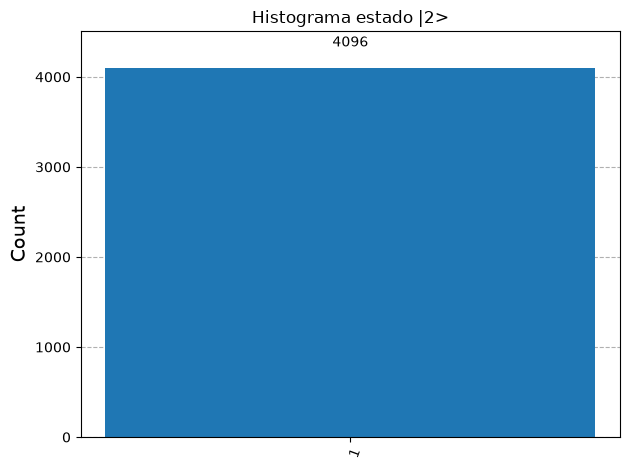
\includegraphics[width=\textwidth]{imagenes/bloque3/e1_histograma_f10.png}
        \caption{}
    \end{subfigure}
    \hfill
    \begin{subfigure}{0.4\textwidth}
        \centering
        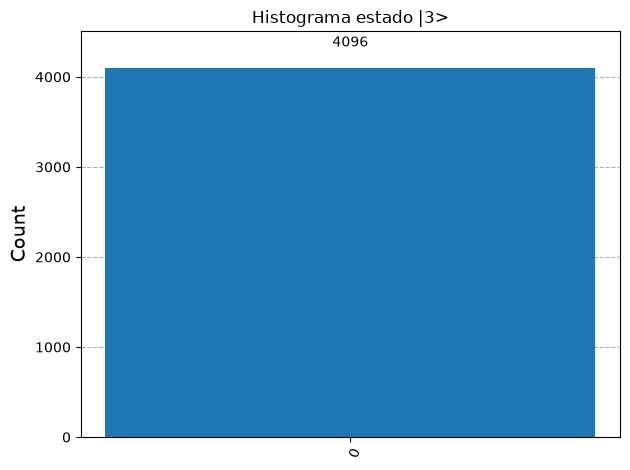
\includegraphics[width=\textwidth]{imagenes/bloque3/e1_histograma_f11.png}
        \caption{}
    \end{subfigure}
    \caption{Resultados de medición sobre $q_2$ tras simular el oráculo $DJ\_F$ para cada uno de las 
    $4$ entradas de la base computacional: $\ket{00}, \ket{01}, \ket{10}$ y $\ket{11}$}\label{fig:bloque3_e1_histogramas}
\end{figure}


El algoritmo de Bernstein--Vazirani trata funciones de la forma
$f(x)=s\cdot x\oplus b$, con $s\in\{0,1\}^n$, $s\cdot x=s_0x_0\oplus s_1x_1$ y
$b\in\{0,1\}$. Se usa el orden $(x_0,x_1)$, con el bit de $q_0$ primero. Del apartado (d),
\[
  f(x_0,x_1)=\overline{x_1}=x_1\oplus 1
  \quad\Longrightarrow\quad s=(s_0,s_1)=(0,1),\qquad b=1 .
\]
Con el auxiliar en $\ket{-}$, el or\'aculo act\'ua por \emph{phase kickback} y, antes de la
$H$ final, el registro de consulta queda en
\[
  \frac{1}{2}\sum_{x}(-1)^{f(x)}\ket{x}
  =(-1)^{b}\,\frac{1}{2}\sum_{x}(-1)^{s\cdot x}\ket{x}
  =(-1)^{b}\,H^{\otimes 2}\ket{s}.
\]
Al aplicar la $H$ final y usar $H^{\otimes 2}H^{\otimes 2}=\mathbb{I}$, el registro queda en
$(-1)^{b}\ket{s}$. De forma equivalente, la amplitud de cada cadena $z$ es
\[
  \alpha_z=\frac{1}{4}\sum_{x}(-1)^{f(x)\oplus z\cdot x}
  =\frac{(-1)^{b}}{4}\sum_{x}(-1)^{(s\oplus z)\cdot x}
  =(-1)^{b}\,\delta_{z,s},
\]
por la ortogonalidad de los caracteres $(-1)^{w\cdot x}$ (la suma vale $4$ si $z=s$ y $0$
en caso contrario). Por tanto:
\begin{itemize}
  \item se mide $z=s$ con probabilidad $|\alpha_s|^2=1$, de modo que la cadena medida en el apartado (b),
        $(c_0,c_1)=(0,1)$, es exactamente el vector $s$ de la f\'ormula obtenida en el apartado(d):
        $s_1=1$ indica que $f$ depende de $x_1$, y $s_0=0$ que no depende de $x_0$;
  \item el t\'ermino $b$ solo aporta una fase global $(-1)^b$ y no se observa en la medici\'on;
  \item el algoritmo devuelve una \'unica cadena porque $f$ es \emph{af\'in}: toda la amplitud
        se concentra en $z=s$. Si $f$ no fuera af\'in, la amplitud se repartir\'ia entre
        varias cadenas;
  \item como $s\neq 00$, se confirma que $f$ es balanceada, de acuerdo con el apartado (c).
\end{itemize}




